\documentclass[10pt,a4paper]{article}
\usepackage{geometry}
\usepackage[french]{babel}
\usepackage[utf8]{inputenc}
\usepackage[T1]{fontenc}
\usepackage{lmodern} \normalfont
\DeclareFontShape{T1}{lmr}{bx}{sc}{<-> ssub * cmr/bx/sc}{}
\usepackage{textcomp}
\usepackage{datetime}
\usepackage{amsmath}
\usepackage{amssymb}
\usepackage{graphicx}
\usepackage{wrapfig}
\usepackage{subcaption}
\usepackage{tocloft}
\usepackage{fixltx2e}
\usepackage{color}
\usepackage[colorlinks=true,
			linkcolor=blue,
			bookmarksnumbered=true,
			pdftitle={Rapport INF2705},
			pdfauthor={Pythagore Deffo, Gwenegan Hudin},
			pdfborder={0 0 0},
			pdfsubject={Rapport de laboratoire INF2705}]{hyperref}

% Custom commands
\newcommand{\HRule}{\rule{\linewidth}{0.5mm}}
\newcommand{\Section}[1]{\section*{#1} \addcontentsline{toc}{section}{#1} \setcounter{subsection}{0}}
%\renewcommand*{\theHsection}{chY.\the\value{section}}
\renewcommand{\thesection}{\Roman{section}.}
\renewcommand{\thesubsection}{\arabic{subsection}.}
\renewcommand{\thesubsubsection}{\alph{subsubsection}.}
\renewcommand{\cftsecnumwidth}{2em}
\renewcommand{\cftsubsecnumwidth}{2em}
\renewcommand{\cftsubsubsecnumwidth}{2em}
\addto\captionsfrench{
	\renewcommand{\cfttoctitlefont}{\Large}
	\renewcommand{\contentsname}{\centering \textsc{Table des Matières}\\[0.5cm]}
}

\renewcommand{\baselinestretch}{1.15}

\begin{document}

\begin{titlepage}
	\begin{center}
		\begin{figure}
        \begin{subfigure}[c]{0.2\textwidth}
        		\centering
                
\includegraphics[width=0.6\textwidth]{images/logo-polymtl}
        \end{subfigure}
		\end{figure}
		
		
		\vspace{30pt}
		\textsc{\huge Génie Informatique}\\
		\textsc{\LARGE Rapport de Travaux Pratiques}\\		
		\vfill
		
		% Title
		\HRule \\[0.7cm]
		{\Huge \bfseries INF4705 - Infographie}\\[0.4cm]
		{\Large Lab 6 : Illumination et aplat de texture}\\[0.2cm]
		\HRule\\[1cm]
		
		\vfill
		
		% Author
		\begin{minipage}{0.49\textwidth}
			\begin{flushleft} \LARGE
				\textbf{Auteurs}\\
				Pythagore Raoul \textsc{Deffo}\\ 1635142\\
				Gwenegan \textsc{Hudin}\\ 1756642\\[0.5cm]
			\end{flushleft}
		\end{minipage}
		\begin{minipage}{0.49\textwidth}
			\begin{flushright} \LARGE
				\textbf{Rendu}\\
				11 Décembre 2014\\ À Polytechnique Montréal\\[0.5cm]
			\end{flushright}
		\end{minipage}
	\end{center}
\end{titlepage}

\newpage

\hfill

\newpage

\tableofcontents

\newpage

\section{Introduction}

Dans ce rapport, nous voulons revenir sur le sixième travail pratique du cours INF2707 - Infographie. Nous aborderons le problème initial, ce que nous avons ou aurions pu ajouter à la réalisation ; après quoi nous discuterons de points précis de notre implémentation, avant d'identifier les difficultés auxquelles nous avons été confrontés.

Pour réaliser ce TP, nous avions 6h de Lab dédiées.

\section{Exposé du problème}

Dans ce TP, nous devions mettre en application les méthodes d'illumination OpenGL évoquées en cours, ainsi que nous essayer à l'application de textures sur un objet 3D.

Les sources fournies au début de ce TP permettaient l'affichage d'une fenêtre OpenGL. Celle-ci présente un modèle 3D de cube, et une pression sur les touches numériques du clavier permet de changer pour un autre modèle (théière, sphère, tore, dodécahèdre, icosahèdre). Une source lumineuse, représentée par une petite sphère, peut être contrôlée avec la souris (position et orientation).

Nos objectifs sont multiples :

\begin{itemize}
	\item Utiliser une source lumineuse en spot, et appliquer les modèles d'illumination de Blinn et Phong par les nuanceurs. Les objets doivent aussi être éclairables sans nuanceurs.
	\item Modifier les paramètres du spot (angle maximal et exposant) par le clavier.
	\item Appliquer une illumination spot à la Direct3D, avec une atténuation sur les bords de la zone éclairée.
	\item Permettre l'illumination d'une des faces du cube sans nuanceur, par subdivision de celle-ci.
	\item Afficher deux textures (dé ou échiquier) sur le cube et la théière. Lorsqu'appliquée au cube, la texture du dé doit effectivement représenter un dé à 6 faces.
	\item Varier le rendu de la texture échiquier en modifiant le mode de répétition sur le cube.
	\item Rendre les pixels noirs transparents par les nuanceurs.
\end{itemize}

Comme pour les travaux précédents, nous avons réalisé ce TP en travaillant avec C++11, dans l'environnement de développement QT Creator 4 sous Fedora.

\section{Ajouts et modifications}

Nous avons respecté les exigences de ce TP sans les altérer.

Si nous avions eu plus de temps, nous aurions pu grandement améliorer notre mécanisme de subdivision de faces, en utilisant des \textit{VertexPointer}. Cela nous aurait permis de gagner en performances, et ainsi mieux subdiviser la face du cube. Cette subdivision pourrait aussi être étendue à toutes les faces du cube.

Cependant, le cube n'était pas le seul modèle à pâtir de l'éclairage OpenGL en pipeline fixe. Ainsi, la division de faces aurait pu être utilisée sur le dodécahèdre et l'icosahèdre. Ceux-ci sont néanmoins bien plus complexes à subdiviser, on ne peut simplement utiliser des \textit{Quads}. Nous aurions eu à nous pencher sur les problématiques de tesselation, et utiliser des triangles.

Enfin, comme nous avions un dé à 6 faces (un d6), il aurait été intéressant d'appliquer des textures similaires pour réaliser un d12 et un d20, respectivement sur le dodécahèdre et l'icosahèdre. Ainsi, nous aurions été parés pour une séance de Donjons \& Dragons !

\section{Discussion}

\subsection{Subdivision de surfaces}

Dans ce travail pratique, nous avons eu à faire une subdivision pour une face d'un cube pour permettre le meilleur éclairage de cette face sans nuanceurs. Pour ce faire, nous nous sommes inspirés d'un algorithme de découpage de surface que nous avons trouvé sur le site suivant:  \href{http://stackoverflow.com/questions/19780788/opengl-c-plain-subdivison-in-quads-radiosity-patches-on-arrays}{Stack Overflow - OpenGL C++ Plain Subdivison in QUADS (Radiosity) patches on arrays}. Quelques difficultés ont été rencontrées, elles seront présentées dans la suite de ce rapport.

\subsection{Illumination}

Nous avons implémenté une lumière orientée de type \textit{spot} pour éclairer les faces d'un cube et d'une théière.  Une lumière ayant un angle maximal (\textit{GL\_SPOT\_CUTOFF}) de projection et un exposant (\textit{GL\_SPOT\_EXPONENT}) modifiables. D'après la loi de Lambert, l'intensité de la lumière et l'angle entre la normale avec la direction des rayons incidents sont liés. Pour ce faire, nous normalisons les surfaces afin qu'elles soient perpendiculaires aux rayons lumineux, ceci pour avoir une réflexion plus intense.

Pour la réflexion spéculaire,  nous avons implémenté deux modèles : celui de Phong dont l'équation est : 
$ cos(\theta) = R \cdot V = reflect (L,N) \cdot V $, et celui de Blinn avec pour équation : $ cos(\theta) = B \cdot N = bissect(L,V) \cdot N $, où $ bissect (L,V) = \frac{L+V}{|L+V|} = normalise(L+V) $. La différence entre les deux modèles est que Phong ajoute les effets spéculaires tandis que Blinn utilise un calcul moins coûteux avec la bissectrice, mais le résultat est presque semblable. (voir les figures ci-dessous).

\begin{figure}[h!]
\centering
	\begin{subfigure}[c]{0.3\textwidth}
		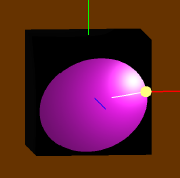
\includegraphics[width=\textwidth]{images/blinn}
		\caption{Eclairage avec le modèle de Blinn}
	\end{subfigure}
	\begin{subfigure}[c]{0.3\textwidth}
		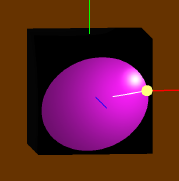
\includegraphics[width=\textwidth]{images/phong}
		\caption{Eclairage avec le modèle de Phong}
	\end{subfigure}
\caption{Différentes méthodes d'éclairage par nuanceur}
\end{figure}

Nous faisons ici un éclairage par fragment à l'aide des nuanceurs pour les deux modèles implémentés. Nous remarquons que pour l'éclairage du cube, les faces qui ne sont pas découpées ne reçoivent d'éclairage qu'à leurs sommets.

Notre programme permet aussi d'alterner entre le modèle \textit{spot} d'OpenGl et le modèle Direct3D.

\subsection{Application de la texture}

La texture étant une image numérique qui recouvre un objet, nous avons appliqué deux différentes textures sur nos objets illuminés : texture de dé et texture d'échiquier. Pour ce faire, nous définissons d'abord les coordonnées des textures, par la suite nous utilisons la fonction \textit{glTexCoordPointer()} qui permet de spécifier la localisation et le format des données des coordonnées de textures que nous utilisons.

\subsection{Forces et faiblesses de l'application}

\subsubsection{Points forts}

\begin{itemize}
	\item Tous les différents modèles d'éclairage implémentés
	\item Textures de base correctement appliquées
	\item Bon outil de subdivision du cube
	\item Effet convaincant sur le mode d'éclairage type Direct3D
\end{itemize}

\subsubsection{Points faibles}

\begin{itemize}
	\item Découpage de surface du cube devrait être fait par \textit{VertexPointer}
	\item Calcul des différents modes de répétition de texture sur le cube
	\item Changement de la transparence des zones noires
\end{itemize}


\section{Difficultés}

\subsection{Subdivision de surfaces}

La subdivision d'une surface du cube a été un des problèmes les plus lourds à gérer durant ce laboratoire, et nous y avons consacré presque la totalité de la première séance (2h30).

Notre premier essai a été le remplissage d'un Vertex Buffer à la main, avec des doubles boucles découpant la face ligne par ligne, tout en respectant le sens horaire de déclaration des sommets. Après de nombreux essais et échecs, ponctués de gels du système, nous nous sommes résolus à chercher des pistes sur Internet.

Nous avons passé un certain temps à lire des documentations et articles, notamment concernant les problématiques de tesselation, qui étaient intéressants mais traitaient de problèmes bien plus complexes que celui que nous voulions résoudre.

Finalement, nous avons trouvé plusieurs question Stack Overflow et posts de forums sur notre problème, dont des méthodes C++11 intéressantes que nous avons utilisé (le lien est cité plus haut, ainsi que dans le \textit{main.cpp} de notre TP). Nous y avons ensuite ajouté le calcul des normales.

\subsection{Compréhension des modèles d'éclairage}

Malgré notre présence durant le cours, et la relecture des notes, les modèles d'illumination de Phong et Blinn restaient encore très obscurs pour nous. Beaucoup de temps a été consacré à la compréhension des formules et de l'importance des variables en jeu, à l'adaptation à une lumière de type \textit{spot}, et au calcul des trois composantes séparées de la lumière.

Il était particulièrement difficile de voir exactement quel résultat lumineux était attendu, donc nous avions l'impression d'avancer dans le flou. Après correction, nous savons que notre méthode d'illumination de Blinn était incorrecte, mais nous ne le voyions pas lors de nos tests. Nous pouvions simplement constater que la composante spéculaire était différente entre Blinn et Phong, et nous paraissait ressembler à l'image d'illumination fournie dans le sujet de laboratoire.

\subsection{Répétition de texture}

Quand nous sommes arrivés au point sur la répétition de texture, nous étions déjà à 10h de travail sur ce laboratoire. Nous avons essayé, empiriquement, d'obtenir l'effet voulu avec ce qu'il nous semblait être les bons paramètres de texture. Le placement (centre, bas gauche...) a été fait par essais successifs jusqu'à trouver des valeurs de multiplication de texture qui semblaient correspondre. Cela ne nous paraissait pas être la bonne méthode, mais nous n'avons pas trouvé d'autre, et l'affichage correspondait avec les images demandées.

Malheureusement, là aussi, suite au retour sur notre TP, nous savons que nous n'avons bel et bien pas fait cela de la bonne façon, mais nous ne voyons toujours pas comment faire.

\section{Conclusion}

Bien qu'il ait été le plus difficile, long et parfois frustrant, ce Lab a aussi été l'un des plus instructifs de ce cours. Nous avons vraiment mieux compris la manipulation de nuanceurs, et l'application de texture, si bien que la réalisation du TP7 a ensuite été très rapide.

Il est cependant dommage de ne pas pouvoir voir les bonnes méthodes que nous aurions dû appliquer sur les points que nous n'avons pas réussi. Peut être serait-il intéressant d'avoir une correction après le TP, ou un retour nous permettant de nous corriger et aussi d'améliorer notre note ?

\end{document}
